\documentclass[11pt]{article}
\usepackage[T1]{fontenc}
\usepackage[paper=letterpaper,margin=1in]{geometry}
\usepackage[parfill]{parskip}
\usepackage{tikz}
\usetikzlibrary{arrows.meta}

\begin{document}
\thispagestyle{empty}

\begin{center}
CS310 -- Assignment 401 -- Karl Ramberg
\end{center}

\textbf{Problem 1:} Given the input 4371, 1323, 6173, 4199, 9679, and
1989 for an initially empty hash table, and the hash function $h(x) =
6 - (x \bmod 7)$, draw the resulting hash table. State and explain any
assumptions you make.

\textit{Answer:}

\begin{center}
% written for clarity, not for efficiency :)
% horizontal coordinates increase left to right
% vertical coordinates increase bottom to top
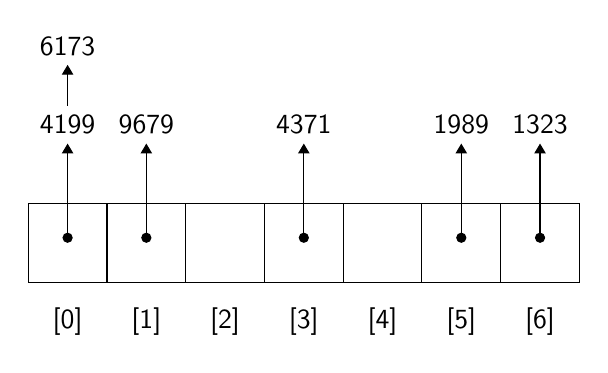
\begin{tikzpicture}[font=\sffamily,scale=0.5]
\draw (0, 0) rectangle (2, 2);
\draw (2, 0) rectangle (4, 2);
\draw (4, 0) rectangle (6, 2);
\draw (6, 0) rectangle (8, 2);
\draw (8, 0) rectangle (10, 2);
\draw (10, 0) rectangle (12, 2);
\draw (12, 0) rectangle (14, 2);
\node (0) at (1, -1) {[0]};
\node (1) at (3, -1) {[1]};
\node (2) at (5, -1) {[2]};
\node (3) at (7, -1) {[3]};
\node (4) at (9, -1) {[4]};
\node (5) at (11, -1) {[5]};
\node (6) at (13, -1) {[6]};
\node (a) at (1, 4) {4199};
\node (b) at (1, 6) {6173};
\node (c) at (3, 4) {9679};
\node (d) at (7, 4) {4371};
\node (e) at (11, 4) {1989};
\node (f) at (13, 4) {1323};
\draw [Circle-Triangle] (1, 1) -- (a);
\draw [Circle-Triangle] (3, 1) -- (c);
\draw [Circle-Triangle] (7, 1) -- (d);
\draw [Circle-Triangle] (11, 1) -- (e);
\draw [Circle-Triangle] (13, 1) -- (f);
\draw [-Triangle] (a) -- (b);
\end{tikzpicture}
\end{center}

\textbf{Problem 2:} Assuming conditions indicate a need to rehash, perform a
rehash the hash table of problem 1, and show the hash table that results from
the rehashing. Briefly explain your process and results.

\textit{Answer:} To rehash we need to increase the table size to the next
prime number more than twice the original size of $7$, which is $17$.
This also means we need to change the hash function to reflect this size to
$h(x) = 16 - (x \bmod 17)$. 

\begin{center}
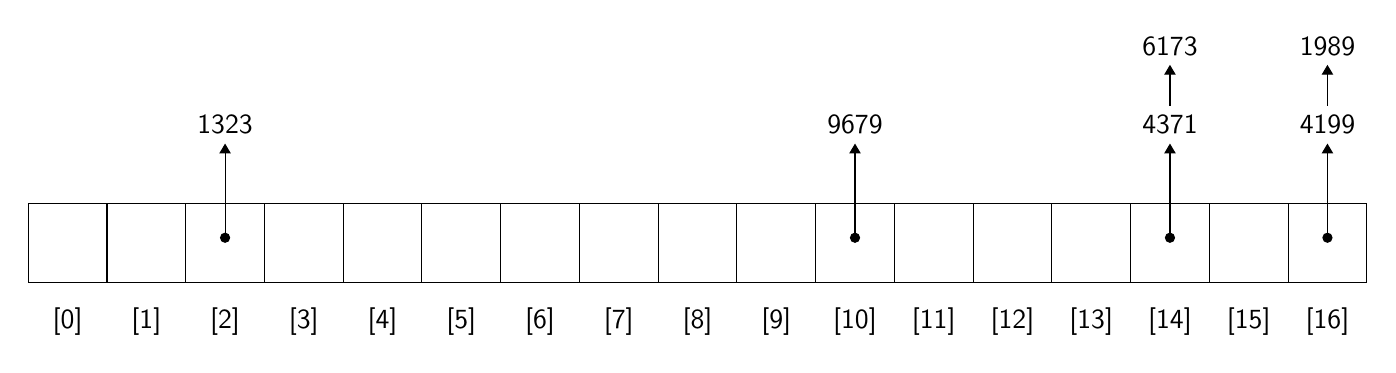
\begin{tikzpicture}[font=\sffamily,scale=0.5]
\draw (0,0) rectangle (2,2);
\draw (2,0) rectangle (4,2);
\draw (4,0) rectangle (6,2);
\draw (6,0) rectangle (8,2);
\draw (8,0) rectangle (10,2);
\draw (10,0) rectangle (12,2);
\draw (12,0) rectangle (14,2);
\draw (14,0) rectangle (16,2);
\draw (16,0) rectangle (18,2);
\draw (18,0) rectangle (20,2);
\draw (20,0) rectangle (22,2);
\draw (22,0) rectangle (24,2);
\draw (24,0) rectangle (26,2);
\draw (26,0) rectangle (28,2);
\draw (28,0) rectangle (30,2);
\draw (30,0) rectangle (32,2);
\draw (32,0) rectangle (34,2);
\node (0) at (1, -1) {[0]};
\node (1) at (3, -1) {[1]};
\node (2) at (5, -1) {[2]};
\node (3) at (7, -1) {[3]};
\node (4) at (9, -1) {[4]};
\node (5) at (11, -1) {[5]};
\node (6) at (13, -1) {[6]};
\node (7) at (15, -1) {[7]};
\node (8) at (17, -1) {[8]};
\node (9) at (19, -1) {[9]};
\node (10) at (21, -1) {[10]};
\node (11) at (23, -1) {[11]};
\node (12) at (25, -1) {[12]};
\node (13) at (27, -1) {[13]};
\node (14) at (29, -1) {[14]};
\node (15) at (31, -1) {[15]};
\node (16) at (33, -1) {[16]};
\node (a) at (5, 4) {1323};
\node (b) at (21, 4) {9679};
\node (c) at (29, 4) {4371};
\node (d) at (29, 6) {6173};
\node (e) at (33, 4) {4199};
\node (f) at (33, 6) {1989};
\draw [Circle-Triangle] (5, 1) -- (a);
\draw [Circle-Triangle] (21, 1) -- (b);
\draw [Circle-Triangle] (29, 1) -- (c);
\draw [-Triangle] (c) -- (d);
\draw [Circle-Triangle] (33, 1) -- (e);
\draw [-Triangle] (e) -- (f);
\end{tikzpicture}
\end{center}

\textbf{Problem 4:} State, explain, and justify the results you got from
running the program in question 3. Be sure to explain what table size you used
in your program, and why you chose that value, and what the load factor used
by your program is. 

\textit{Answer:} I am using Solus Linux distro and when I ran
\texttt{\$ wc -w /usr/share/dict/words} I got a word count of $1,931,546$. For
my program I used a table size of $2,000,000$. This means I have a load factor
($\alpha$) of $0.965773$ which is close to $1$. The total number of collisions
was $691,914$.
\end{document}